\documentclass[smallextended]{svjour3}

\usepackage[utf8]{inputenc}

%\title{A note on conflict set generation\\ for congruence closure\\\small Extended abstract}
%\titlerunning{A note on congruence closure}
\title{NP-completeness of small conflict set generation for congruence closure\thanks{This work has been partially supported by the project ANR-13-IS02-0001 of the Agence Nationale de la Recherche, by the H2020-FETOPEN-2016-2017-CSA project SC$^2$ (712689), by an ÖAW APART Stipendium, by FWF S11407-N23 (RiSE/SHiNE), by ERC Start Grants Graph Games (279307) and  Matryoshka (713999), and by FFG project number 845582 (TRUCONF).}}
\titlerunning{NP-completeness of small conflict set generation for congruence closure}


\author{Andreas Fellner%\inst{1,2}
   \and Pascal Fontaine%\inst{3}
   %\and\\ Georg Hofferek\inst{4}
   \and Bruno Woltzenlogel Paleo%\inst{2,5}
}
\institute{
A. Fellner \at
  Austrian Institute of Technology and
  Vienna University of Technology (Austria)\\
        \email{andreas.fellner@ait.ac.at}
\and
P. Fontaine \at
  Inria, Loria, U. of Lorraine (France)
\and
B. Woltzenlogel Paleo \at
  Vienna University of Technology (Austria) and
  Australian National University (Australia)
}

\date{Received: date / Accepted: date}

\authorrunning{Fellner et al.}

\journalname{Formal Methods in System Design - Recent topics in SMT}

\usepackage[utf8]{inputenc}
\usepackage[T1]{fontenc}
\usepackage{lmodern}

\usepackage{amssymb}
\usepackage{amsmath}
\usepackage{graphicx}                                   % Figures
\usepackage{tikz}                                       % tikz graphics
\usetikzlibrary{arrows,automata,positioning}
\usetikzlibrary{fit}
%\usepackage{hyperref}

%\newtheorem{example}{Example}
%\newtheorem{definition}{Definition}
%\newtheorem{corollary}{Corollary}
%\newtheorem{theorem}{Theorem}
%\newtheorem{lemma}{Lemma}
%\newtheorem{proposition}[theorem]{Proposition}

\def\proofname{Proof.}%

\newcommand{\Assignment}{{\it AssignmentEqs}}
\newcommand{\Clause}{{\it Clause}}
\newcommand{\Connect}{{\it Connect}}

\begin{document}

\maketitle

\begin{abstract}
The efficiency of Satisfiability Modulo Theories (SMT) solvers is dependent on the capability of theory reasoners to provide small conflict sets, i.e.\ small unsatisfiable subsets from unsatisfiable sets of literals.  Decision procedures for uninterpreted symbols (i.e.\ congruence closure algorithms) date back from the very early days of SMT.  Nevertheless, to the best of our knowledge, the complexity of generating smallest conflict sets for sets of literals with uninterpreted symbols and equalities had not yet been determined, although the corresponding decision problem was believed to be NP-complete. We provide here an NP-completeness proof, using a simple reduction from SAT.
\keywords{Satisfiability Modulo Theories \and Decision procedures \and Congruence closure \and Complexity}
\end{abstract}


\section{Introduction}

Satisfiability Modulo Theory solvers are nowadays based on a cooperation between a
propositional satisfiability (SAT) solver and a theory reasoner for the
combination of theories supported by the SMT solver. The propositional
structure of the problem is handled by the SAT solver, whereas the theory
reasoner only has to deal with conjunctions of literals.  Very schematically (we
refer to~\cite{Barrett14} for more details) the Boolean abstraction of the SMT
problem is repeatedly refined by adding theory conflict clauses that eliminate
spurious models of the abstraction, until either unsatisfiability is reached, or
a model of the SMT formula is found.  Refinements can be done by refuting models
of the propositional abstraction one at a time.  It is, however, much more
productive to refute all propositional models that are spurious for the same
reason at once.  A model of the abstraction is spurious if the set of concrete literals
corresponding to the abstracted literals satisfied by this model is
unsatisfiable modulo the theory.  Given such an unsatisfiable set of concrete literals, the
disjunction of the negations of any unsatisfiable subset (a.k.a. \emph{core}) is a suitable
conflict clause.  By backtracking and asserting the conflict clause, the
SAT-solver is prevented from generating the spurious model again. The smaller
the clause, the stronger it is and the more spurious models it prevents.
Therefore, an optimal conflict clause, corresponding to a minimal unsatisfiable
subset of literals (i.e.\ such that all its proper subsets are satisfiable) or
even a minimum one (i.e.\ smallest among the minimals) is desirable.  This
feature of the theory reasoners to \emph{generate small conflict sets} (a name
adopted in~\cite{Barrett14}) from their input is also referred to as \emph{proof
production}~\cite{Nieuwenhuis3,Nieuwenhuis9} or \emph{explanation
generation}~\cite{Nieuwenhuis6}.
%% \marginpar{TODO: This footnote is vague. I would suggest removing it. ``unuseful'' doesn't exist, but ``useless'' would sound too strong. }\footnote{\emph{Proof production} and \emph{explanation
%%   generation} additionally convey the idea that, besides giving a small
%%   unsatisfiable subset, the valuable reasoning process can be isolated from the
%%   unuseful computation.}

Decision procedures for the theory of uninterpreted symbols and equality can be
based on congruence closure~\cite{Nelson2,Downey1,Nieuwenhuis6}.  The decision problem is polynomial
and even quasi-linear~\cite{Downey1} with respect to the number of terms and
literals in the input set.  Producing minimal conflict sets also takes
polynomial time.  Indeed, testing if a set $S$ remains unsatisfiable after
removal of one of its literals is also polynomial.  It suffices then to
repeatedly test the $|S|$ literals of $S$ to check if they can be removed.  The
set $S$ pruned of its unnecessary literals is minimal.  One could also profit from 
the incrementality of the decision procedure~\cite{Fontaine1}.

It has also been common knowledge that computing minimum conflict clauses for
the theory of uninterpreted symbols and equality is a difficult problem.  But,
to our best knowledge, the complexity of finding the smallest conflict clause generation
for sets of literals with uninterpreted symbols and equalities has never been
established.  The complexity of the corresponding decision problem (i.e. of whether there exists a conflict clause with size smaller than a given $k$) is mentioned to be NP-complete in~\cite{Nieuwenhuis6} --- with
a reference to a private communication with Ashish Tiwari --- but neither the
authors of~\cite{Nieuwenhuis6} nor Ashish Tiwari published a written proof of
this fact\footnote{We contacted both Ashish Tiwari and the authors
  of~\cite{Nieuwenhuis6}, who confirmed this.}.

Our interest in this problem arose from our work on Skeptik \cite{Boudou1}, a tool for the compression of proofs generated by SAT and SMT solvers. For the sake of moving beyond the purely propositional level, we have developed an algorithm for compressing congruence closure proofs, which consists of regenerating (possibly smaller) congruence closure conflict clauses while traversing the proof. 
Congruence closure conflict clauses are typically generated from paths in the \emph{congruence graph} maintained by the congruence closure algorithm \cite{Fontaine2004,Nieuwenhuis6,Nieuwenhuis9}. 
In order to obtain small conflict clauses, and thereby small congruence closure proofs, we (dynamically) assigned weights to the congruence graph and searched for shortest paths in that graph.
The weights of input equations would be $1$, whereas the weight of a congruence edge would be the size of an explanation of its equation.
This raised the question whether we could construct shortest conflict clauses as shortest paths in such weighted congruence graphs, by applying a polynomial time shortest path algorithm to a graph of polynomial size.
We answered this question negatively by proving that the problem of deciding whether a shorter conflict clause exists is NP-hard. 
The goal of this article is to present this proof.
The reason why the shortest path method is not able to find shortest conflict clauses is that the weights for congruence edges can not be accurately determined a priori.
A preliminary version was presented at the SMT Workshop 2015~\cite{Fellner1}.

\section{Preliminaries}

We assume knowledge of propositional logic and quantifier-free first-order logic
with equality and uninterpreted symbols, and only enumerate the notions and
notations used in this article.
%TODO Propositional logic studies formulas written  $\vee$, $\wedge$, $\neg$
A literal is either a propositional variable or the negation of a propositional
variable.  A clause is a disjunctive set of literals.  A propositional variable
$x$ appears positively (negatively) in a clause $C$ if $x \in C$ (resp.\ $\neg x
\in C$).  The notations $\{\ell_1, \dots \ell_n\}$ and $\ell_1 \vee \dots \vee
\ell_n$ will be used interchangeably.  A clause is tautological if and only if it contains a
variable both positively and negatively.  We
shall tacitly assume that clauses are non-tautological, except when explicitly stated otherwise.
Clauses being sets, they cannot contain multiple occurrences of the same
literal.  A formula in conjunctive normal form (CNF for short) is a conjunctive
set of clauses.  A total (partial) assignment $\cal I$ for a formula in
propositional logic assigns a value in $\{\top, \bot\}$ to each (resp.\ some)
propositional variable(s) in the formula.  An assignment $\cal I$ for a formula
$F$ is a model of $F$, denoted ${\cal I}\models F$, if it makes the formula $F$
true.  A formula is satisfiable if it has a model, it is unsatisfiable
otherwise.  A total or partial assignment is perfectly defined by the set of
literals it makes true.  By default, an assignment is total unless explicitly
said to be partial.  A set of formulas $E$ entails a (set of) formula(s) $E'$,
denoted $E\models E'$, if every model of $E$ is a model of $E'$.


%\vspace*{5pt}
%\noindent \textbf{Congruence closure and congruence graph}

%\noindent
%We do not give here a full description of congruence closure algorithms and
%refer the reader to~\cite{Nelson2,Downey1,Nieuwenhuis6} for more details.  We
%only remind that the satisfiability of a set of first-order literals with
%equality and uninterpreted symbols $E$ can easily be checked by building a
%congruence graph.
%We denote the set of all terms and subterms occurring in $E$ by $\mathcal{T}(E)$.
%A congruence graph is built on a set of nodes including (but
%not restricted to) $\mathcal{T}(E)$.  
%%We assume this set of nodes
%%is finite, and unless stated otherwise, only contains the terms and subterms in
%%$E$. 
%Throughout this work, we assume that when we check whether $E \models s = t$, it is the case that $s,t\in \mathcal{T}(E)$.
%Under this assumption, the set of nodes in the congruence graph are restricted to $\mathcal{T}(E)$.
%The assumption is w.l.o.g. since if $s \notin \mathcal{T}(E)$ we can add the tautological equations $s=s$ to $E$ and likewise for $t$ (e.g. when deducing $f(a) = f(b)$ from $\{a=b\}$).
%Adding these equations does not change the congruence closure of $E$ and only adds a constant number of equations.
%
%There are two kinds of edges in the graph: full edges and congruence edges.
%There is a full edge between two nodes associated with terms $s$ and $t$ if and
%only if there is an equality $s=t$ (or $t=s$) in $E$.  The congruence closure
%algorithm adds congruence edges to the graph until (the smallest) fix-point is
%reached: a congruence edge is added between two terms with the same top symbol
%$f(s_1, \dots s_n)$ and $f(t_1, \dots t_n)$ if there is a path (using full and
%congruence edges) from $s_i$ to $t_i$ for all $i\in \{1,\dots n\}$.  An equality
%$s=t$ between two terms in $E$ is implied by a set of literals $E$ if and only if
%there is a path between $s$ and $t$ in the congruence graph of $E$.  A set of
%first-order literals $E$ is unsatisfiable if and only if there is an inequality
%$s\neq t \in E$ such that there is a path between $s$ and $t$ in the congruence
%graph of $E$.

%In this section we define the concepts of congruence- relation and closure, which is the foundation of our proof compression method.
%To this end we define terms and equations, which are notions that will be used throughout this chapter.
%We close this section by proving some elementary properties of congruence relations.

We now define the necessary notions for quantifier-free first-order logic.
\begin{definition}[Terms and equations]
A \emph{signature} $\Sigma$ is a finite set of function symbols $\mathcal{F}$
equipped with an \emph{arity} function $\mathcal{F} \rightarrow \mathbb{N}$.  A
\emph{constant} is a nullary function.  A \emph{unary} function has
arity one.  Given a signature $\Sigma$, the set of \emph{terms}
$\mathcal{T}^{\Sigma}$ is the smallest set containing all constants in
$\mathcal{F}$ and all terms of the form $g(t_1,\ldots, t_n)$, where $g$ is a
function symbol of arity $n$ in $\mathcal{F}$ and $t_1,\ldots,t_n$ are terms in $\mathcal{T}^{\Sigma}$.  An \emph{equation} between two terms $s,t$ in $\mathcal{T}^{\Sigma}$ is denoted by $s=t$.
\end{definition}
Signatures commonly include predicate symbols.  Everything extends smoothly to
signatures with predicates, but to simplify, a quantifier-free first-order logic
formula is here just a Boolean combination of equalities between terms; a
literal is either an equation or the negation of an equation.

The terms $t_1,\ldots,t_n$ are \emph{direct subterms} of $g(t_1,\ldots,t_n)$.  The \emph{subterm} relation is the reflexive and transitive closure of the direct subterm relation.
Given a set of equations $E$, we denote by $\mathcal{T}(E)$ the set of terms and subterms occurring in the equations.

An assignment ${\cal I}$ on some signature maps each constant to an element in a
universe $\mathcal{U}$, and each function symbol to a function of appropriate
arity on $\mathcal{U}$.  By extension, it assigns an element in $\mathcal{U}$ to
every term, and a value to every equation $s=t$, namely $\top$ if
$\mathcal{I}(s) = \mathcal{I}(t)$ and $\bot$ otherwise.  Like in propositional
logic, an assignment on some signature thus gives a truth value to every
formula on this signature.

%Our definition of terms corresponds to what is usually called ground term in the context of first order logic.
%Ground terms are terms that contain no first order logic variables.
%Since we do not investigate non ground terms, we omit the complement and simply speak of terms.
%
%\noindent Should $\Sigma$ be clear from context or of no relevance, we will omit it and write $\mathcal{T}$ instead of $\mathcal{T}^{\Sigma}$.
%
%\newpage
\begin{definition}[Congruence relation]  Given a set of terms $\mathcal{T}$ closed under the subterm relation, a relation $R \subseteq \mathcal{T} \times \mathcal{T}$ is a congruence if it is
\begin{itemize}
\item reflexive: $(t,t) \in R$ for each $t \in \mathcal{T}$;
\item symmetric: $(s,t) \in R$ if $(t,s) \in R$;
\item transitive:  $(r,t) \in R$ if $(r,s) \in R$ and $(s,t) \in R$;
\item compatible: $(g(t_1,\ldots,t_n),g(s_1,\ldots,s_n)) \in R$ if  $g$ is a $n$-ary function symbol and $(t_i,s_i) \in R$  for all $i = 1,\ldots,n$.
\end{itemize}

\end{definition}
\noindent A congruence relation is also an equivalence relation, since it is
reflexive, transitive and symmetric.  Therefore a congruence relation partitions
its underlying set of terms $\mathcal{T}$ into congruence classes, such that two
terms $(s,t)$ belong to the same class if and only if $(s,t) \in R$.  The
relations $\left\{{\left({t, t}\right): t \in \mathcal{T}}\right\}$ and $\mathcal{T} \times \mathcal{T}$ are trivial
congruence relations.  An assignment $\cal I$ on a signature $\Sigma$ defines a congruence relation on any subset $\mathcal{T}\subseteq\mathcal{T}^\Sigma$, that is, $R = \{(s,t) \ |\ \mathcal{I}(s = t) = \top \}$.

An equation $s = t$ on terms in a set $\mathcal{T}$ can be seen as a singleton relation $\{(s,t)\} \subseteq \mathcal{T} \times \mathcal{T}$.  By extension, a set of equations can also be seen as a relation, i.e., the union of the singleton relations. 
%In this work we are interested in congruence relations induced by sets of equations.
%In other words, we compute the partitioning of the terms such that two terms in the same partition are proven to be equal by the input set of equations.
%To this end we define the notion of congruence closure of a set of equations.

\begin{definition}[Congruence closure]
The congruence closure $E^*$ of a set of equations $E$ on a set of terms $\mathcal{T}$ closed under the subterm relation is the smallest congruence relation on $\mathcal{T}$ containing $E$.
%We call a pair $(s,t)$ in a congruence closure an \emph{equality} and we call an equality of compound terms $(g(t_1,\ldots,t_n),g(s_1,\ldots,s_n))$ such that for all $i = 1,\ldots,n$: $E \models t_i \thickapprox s_i$ a \emph{deduced equality}.
%For a term $t \in \mathcal{T}_E$ the set of congruent terms $\{s \in \mathcal{T}_E \mid E \models s \thickapprox t\}$ is the \emph{congruence class} of $t$.

\end{definition}
\noindent
Since congruence relations are closed under intersection, the congruence closure of a set of equations always exists.  Also notice that, if  $(s,t) \in E^*$, then $E \models s = t$.  We say that $E$ is an \emph{explanation} for $s = t$.

An algorithm computing the congruence closure of a relation is also a decision procedure for the problem of satisfiability of sets of equalities
and disequalities in quantifier-free first-order logic with uninterpreted
(predicates and) functions.  It suffices indeed to compute the congruence
closure of all equalities on the terms and subterms occurring in the
literals.
Then, the set of literals is satisfiable if and only if there is no disequality with both terms in the same class.  A model can be built from the congruence closure, on a universe with cardinality equal to the number of classes in the congruence.

%\begin{proposition}[Properties of the $\models$ relation]
%\label{prop:models}
%The $\models$ relation is monotone: $E_1 \subseteq E_2$ and $E_1 \models s \thickapprox t$ implies $E_2 \models s \thickapprox t$ and consistent: $E \models s \thickapprox t$ and $E \cup \{(s,t)\} \models u \thickapprox v$ implies $E \models u \thickapprox v$. 
%
%\end{proposition}
%
%\begin{proof}
%
%Monotonicity follows from the fact that congruence closure of $E_1$ is contained in the congruence closure of $E_2$.
%
%Since the congruence closure of $E^*$ is $E^*$ itself, it follows that $E \models u \thickapprox v$ if and only if $E^* \models u \thickapprox v$.
%Since $(s,t) \in E^*$, clearly it is the case that $E^* = (E \cup \{(s,t)\})^*$.
%Therefore $E \cup \{(s,t)\} \models u \thickapprox v$ implies $(u,v) \in E^*$, i.e. $E \models u \thickapprox v$ or in other words, the $\models$ relation is consistent.
%
%\end{proof}

\section{Congruence Closure in Practice}

The algorithms we consider in the following take as input a set of literals $E$.
Considering complexity, not only the cardinality of the set is important, but
also the number of terms and subterms as well as the number of their
occurrences.  Congruence closure algorithms in modern SMT solvers typically
represent terms with Directed Acyclic Graphs (DAGs) using maximal sharing, and
not trees.  The number of term and subterm occurrences does not matter, but only
the number of distinct (sub)terms.  The input is also typically not a set, but
successive calls to an assertion function with a literal as argument: every
repetition of the same literal then matters for complexity.  Let us assume,
however, that the input is a set $E$, terms are DAGs with maximal
sharing (i.e. identity of atomic symbols and complex terms can be checked in constant time). Therefore, we
characterize complexity results in terms of number of literals, terms and
subterms of the input set, i.e. $|E|$ and $|\mathcal{T}(E)|$.

Since congruence relations are basically partitions of equivalent terms that
additionally satisfy the compatibility property, it is unsurprising that
practical congruence closure algorithms, or decision procedures for ground sets
of first-order logic literals, are based on some kind of union-find
data-structure.  Terms (and subterms) are put into equivalence classes,
according to the equalities in the input.  The algorithms furthermore check,
every time two classes of the partition are merged, whether any new equality induced
by compatibility has to be taken into account.  Also, it checks that the
congruence is consistent with the set of disequalities.  We refer the reader
to~\cite{Nelson2,Downey1,Nieuwenhuis6} for more details.  The complexity of
those algorithms depend on the internal data-structures and on the
representation of terms~\cite{Downey1}.  Algorithms typically implemented in SMT
solvers have complexity $\mathcal{O}(|E| + (|\mathcal{T}(E)| \cdot \log
|\mathcal{T}(E)|))$ assuming constant time operations on the hash table being used to detect new equalities induced by compatibility.

The generation of conflict sets or explanations is based on the congruence
graph: its nodes are the terms and subterms considered by the algorithm.  An
edge in the graph is either a full edge, linking two nodes $s$ and $t$ and
labeled by an input equation $s=t$, or a congruence edge (a dotted edge in the
figures in this article), linking two terms with the same leading function symbol
and labeled by the compatibility-deduced equality between both terms.  The graph
has a path between two terms if and only if they belong to the same congruence
class.  The equality between two terms in the same class is a logical consequence
of the set of equations labeling the path.  To get an explanation for the
equality of two terms in the same class, that is, a set of input equations
implying the equality of the two terms, it thus suffices to collect the set of
equations labeling a path, and recursively replace any compatibility equation
$g(t_1,\ldots,t_n) = g(s_1,\ldots,s_n)$ by the explanations of $t_1=s_1$,\dots,
$t_n=s_n$.

\begin{figure}[ht]

\centering
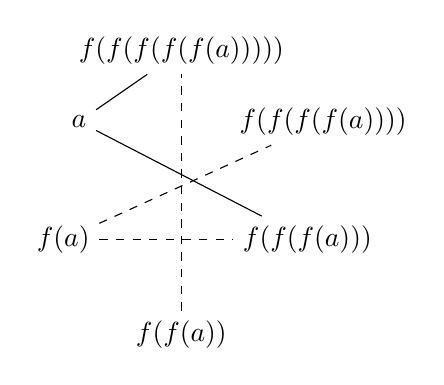
\begin{tikzpicture}[node distance=.3cm]

\node(a){$a$};
\node[below =1cm of a, xshift = -0.2cm] (f1a) {$f(a)$};
\node[below =0.6cm of f1a, xshift = 1.5cm] (f2a) {$f(f(a))$};
\node[right =2cm of f1a, xshift = -0.3cm] (f3a) {$f(f(f(a)))$};
\node[right =2cm of a, xshift = -0.3cm] (f4a) {$f(f(f(f(a))))$};
\node[above =3cm of f2a] (f5a) {$f(f(f(f(f(a)))))$};

%% \draw [-] (a) to (f1a);
%% \draw [-] (f1a) to (f2a);
%% \draw [-] (f2a) to (f3a);
%% \draw [-] (f3a) to (f4a);
%% \draw [-] (f4a) to (f5a);
%% \draw [-] (f5a) to (a);

\draw [-] (a) to (f3a);
\draw [-] (a) to (f5a);
\draw [dashed] (f1a) to (f4a);
\draw [dashed] (f2a) to (f5a);
\draw [dashed] (f1a) to (f3a);

%% \draw [-] (c1) to (f1x3);


%% \node[right =.4cm of t1x1, yshift = 0.25cm] (f11) {$f_1(\bot_1)$};
%% \node[above =.4cm of f11] (t11) {$t_1(\top_1)$};
%% \node[below =.4cm of f11] (t12) {$t_1(\top_2)$};
%% \node[below =.4cm of t12] (f12) {$f_1(\bot_2)$};
%% \node[below =.4cm of f12] (t13) {$t_1(\top_3)$};
%% \node[below =.4cm of t13] (f13) {$f_1(\bot_3)$};

%% \node[right = 4cm of c1](c2){$\hat{c}_2$};

%% \draw [-] (c2) to (t11);
%% \draw [-] (c2) to (t12);
%% \draw [-] (c2) to (t13);
%% \draw [-] (c2) to (f11);
%% \draw [-] (c2) to (f12);
%% \draw [-] (c2) to (f13);

%% \node[right =.25cm of c2, yshift=1cm]  (f2x2) {$f_2(\hat{x}_2)$};
%% \node[below =1.5cm of f2x2] (t2x3) {$t_2(\hat{x}_3)$};

%% \draw [-] (c2) to (f2x2);
%% \draw [-] (c2) to (t2x3);

%% \node[right =3cm of f11] (f21) {$f_2(\bot_1)$};
%% \node[right =3cm of t11] (t21) {$t_2(\top_1)$};
%% \node[right =3cm of t12] (t22) {$t_2(\top_2)$};
%% \node[right =3cm of f12] (f22) {$f_2(\bot_2)$};
%% \node[right =3cm of t13] (t23) {$t_2(\top_3)$};
%% \node[right =3cm of f13] (f23) {$f_2(\bot_3)$};

%% \node[right = 4cm of c2](c3){$\hat{c}_3$};

%% \draw [-] (c3) to (t21);
%% \draw [-] (c3) to (t22);
%% \draw [-] (c3) to (t23);
%% \draw [-] (c3) to (f21);
%% \draw [-] (c3) to (f22);
%% \draw [-] (c3) to (f23);

%% \node[right =.25cm of c3, yshift=1cm] (f3x1) {$f_3(\hat{x}_1)$};
%% \node[below =1.5cm of f3x1] (f3x2) {$f_3(\hat{x}_2)$};

%% \draw [-] (c3) to (f3x1);
%% \draw [-] (c3) to (f3x2);

%% \node[right =3.4cm of f21] (f31) {$f_3(\bot_1)$};
%% \node[right =3.4cm of t21] (t31) {$t_3(\top_1)$};
%% \node[right =3.4cm of t22] (t32) {$t_3(\top_2)$};
%% \node[right =3.4cm of f22] (f32) {$f_3(\bot_2)$};
%% \node[right =3.4cm of t23] (t33) {$t_3(\top_3)$};
%% \node[right =3.4cm of f23] (f33) {$f_3(\bot_3)$};

%% \node[right = 4.5cm of c3](c4){$\hat{c}_4$};

%% \draw [-] (c4) to (t31);
%% \draw [-] (c4) to (t32);
%% \draw [-] (c4) to (t33);
%% \draw [-] (c4) to (f31);
%% \draw [-] (c4) to (f32);
%% \draw [-] (c4) to (f33);

\end{tikzpicture}


\caption{An example congruence graph}
\label{fig:congruenceexample}
\end{figure}

\begin{example}
A congruence graph for two input equations $a = f(f(f(a)))$ and $a =
f(f(f(f(f(a)))))$ is given on Figure~\ref{fig:congruenceexample}.  Labeling
equations are omitted for simplicity.  There is a path between $a$ and $f(a)$,
so both terms are equal if the input equations hold.  To compute an explanation
for $a=f(a)$, it suffices to collect the equalities on the path, that is, the
input equation $a=f(f(f(a))))$ and the compatibility equation $f(a)=f(f(f(a)))$.
This last equation should then be replaced by the equation between the
arguments, i.e., $a=f(f(a)))$ which is consequence, by transitivity, of another
compatibility equation and of the other input equation $a = f(f(f(f(f(a)))))$.
Hence the explanation will contain both equations.
\end{example}



Practical congruence closure algorithms with explanation build a congruence
graph while computing the congruence closure.  Every time the decision procedure
merges two classes, either because of an input equation or because an equality was deduced due to compatibility,
a full- or congruence- edge is added to the graph.  
Since edges between nodes are only added when their respective congruence classes are merged, 
the path between two terms in the same class is unique.  The
explanation that two terms are equal is also unique, but there is no guarantee
that this explanation is the smallest one.  Indeed, it may happen that the
algorithm considers, e.g.\ equations $a=b$ and $b=c$ before $a=c$, merging $a$,
$b$ and $c$ before considering the last equation, and thus discarding $a=c$ as
redundant: in that case, $a=c$ would have been the smallest proof that $a$ and
$c$ are equal, but the congruence graph would only consider the two other
equalities. 
There is not even a guarantee that the explanation is minimal.
Again, the congruence closure algorithm can prove that $a = f(b)$ from the input
equations $b = f(a)$, $f(a) = f(b)$ and $a = b$.
The redundant equality $f(a) = f(b)$
would be recorded in the congruence graph, and thus be part of the explanation, if it is considered before $a = b$.

In practice, the congruence closure procedures implemented in SMT solvers
produce explanations efficiently: the complexity of the explanation production
is quasi-linear with respect to the explanation size, which is at most equal to
the size of the input~\cite{Nieuwenhuis6}.  But the explanations are not optimal, i.e.\ they are not always the smallest. In fact, they are not even minimal. It is possible to compute minimal
explanations in polynomial time; it suffices for instance to compute again the
congruence closure iteratively removing every equation in the explanation, to
see if it is redundant or not. One could (naively) hope to conceive a different
congruence closure algorithm generating the smallest explanation in polynomial
time. For example, one might attempt to modify the iterative removal algorithm; or attempt to modify shortest path algorithms and apply them to congruence graphs enriched with redundant equations as labels. However, such attempts would be futile. As proven in the next section, the corresponding decision problem is NP-hard. 


\section{NP-Completeness of the Small Conflict Set Problem}
\label{sec:npcomplete}

%% Rather than considering directly the conflict set generation problem ---
%% given a natural number $k$ and an unsatisfiable set of literals, is there a
%% conflict set with size smaller than $k$ --- we will rather work on the small
%% explanation problem: given a natural number $k$ a set of equalities $E$ and
%% an equality $s=t$ is there a subset of $E$ smaller than $k$ that implies a
%% given equality $s=t$.

%Let us first define the small conflict set generation problem formally:

The function problem of \emph{generating} the smallest conflict set corresponds to 
the decision problem of \emph{deciding} whether a conflict set with 
size smaller than a given $k$ exists.

\begin{definition}[Small conflict set problem]
Given an unsatisfiable set $E$ of literals in quantifier-free first-order logic
with equality and $k \in \mathbb{N}$, the \emph{small conflict set generation
  problem} is the problem of deciding whether there exists an unsatisfiable set
$E' \subseteq E$ with $|E'| \leq k$.
\end{definition}

\noindent If we had a polynomial-time algorithm $\alpha$ capable of generating 
the smallest conflict set for any unsatisfiable set $E$, 
then we could decide in polynomial time any instance of the small conflict set 
problem by applying $\alpha$ to $E$ and checking whether $\alpha(E)$ has size smaller than $k$. 
However, as proven below, the small conflict set problem is NP-complete and, therefore, 
polynomial time generation of conflict sets with minimum size is not possible (unless P = NP).
%
Our proof reduces the problem
of deciding the satisfiability of a propositional logic formula in conjunctive
normal form (SAT) to the small explanation problem.
%
\begin{definition}[Small explanation problem]
Given a set of equations $E = \{ s_1=t_1,\ldots s_n=t_n\}$, $k \in
\mathbb{N}$ and a target equation $s = t$, the \emph{small explanation problem}
is the problem of answering whether there exists a set $E'$ such that $E'
\subseteq E$, $E' \models s = t$ and $|E'| \leq k$.
\end{definition}

%\marginpar{In this paragraph, we are assuming that $=$ is the only predicate symbol. But we have not stated this assumption before. }
% PF2whoever: I think this is not a problem.
\noindent The small explanation problem and the small conflict set
problem are closely related: there is a small explanation of size $k$ of $s=t$
from $E$ if and only if there is a small conflict of size $k+1$ for $E \cup
\{s\neq t\}$.  
%The proof of hardness is based on a (polynomial) translation of
%the propositional satisfiability problem to the small explanation problem.


In the following we describe a polynomial translation from instances of the propositional satisfiability problem to instances of the small explanation problem.
The translation consists of two
parts: a translation of propositional formulas, here assumed, without loss
of generality, to be in CNF (as shown in Definition \ref{def:CNFCongruenceTranslation}), and a translation of assignments (as shown in Definition \ref{def:AssignmentCongruenceTranslation}).


\begin{definition}[CNF congruence translation]
\label{def:CNFCongruenceTranslation}
Let $\mathcal{C}$ be a set of propositional clauses $\{C_1,\ldots C_n\}$ using variables $x_1,\ldots,x_m$.
%The set of terms $\mathcal{T}$ is constructed using the following constants and function symbols.
%For every $i= 1,\ldots,n + 1$, there is a constant $\hat{c}_i$ and function symbols $t_i$ and $f_i$.
%For every $j= 1,\ldots,m$, there are constants $\hat{x}_j$, $\top_j$ and $\bot_j$.
The \emph{congruence translation} $E_{\mathcal{C}}$ of\/ $\mathcal{C}$ is defined as the set of equations
\begin{equation*}
E_{\mathcal{C}} = \Connect \cup \bigcup_{1 \leq i \leq n}\Clause_i 
\end{equation*}
with
\begin{eqnarray*}
        \Connect &=& \{ c_{i}' = c_{i+1} \ \mid\ 1 \leq i < n\}\\
        \Clause_i &=& \{ c_i = t_i(\hat{x}_j) \ \mid\ x_j \text{ appears in } C_i \}\\
           & & \cup\ \{ t_i(\top_j) = c_i' \ \mid\ x_j \text{ appears positively in } C_i \}\\
           & & \cup\ \{ t_i(\bot_j) = c_i' \ \mid\ x_j \text{ appears negatively in } C_i \}
\end{eqnarray*}
where $c_{1},\dots c_{n},c_{1}', \dots c_{n}',
\hat{x}_1, \dots \hat{x}_m, \top_1, \dots \top_m, \bot_1, \dots \bot_m$ are distinct constants, and $t_1, \dots t_n$ are
distinct unary functions.\footnote{It would be possible to define a translation without the $c_i'$ constants, but they ease the presentation.}
\end{definition}

\begin{remark}
Note that the constants $\top_i$ and $\bot_i$ (for $1 \leq i \leq m)$) should not be confused with the Boolean values $\top$ and $\bot$. The intuitive relationship between these constants and the boolean values is established in Definition \ref{def:AssignmentCongruenceTranslation}.
\end{remark}


\noindent The translation of clauses is illustrated by the following example.
% and a subset of the translation corresponding to a satisfying assignment.
%We use the standard notion of satisfiability and present variable assignments as sets of those propositional variables being mapped to true.

\begin{example}\label{ex:np1}
Consider the set of clauses $\mathcal{C}$
\begin{equation*}
\big\{C_1 = x_1 \vee x_2 \vee \neg x_3, C_2 = \neg x_2 \vee x_3, C_3 = \neg x_1 \vee \neg x_2\big\}.
\end{equation*}
Figure~\ref{fig:npexamplebig} represents the congruence translation of
$\mathcal{C}$ graphically, an edge between two nodes meaning that the set
contains an equation between the terms labeling the two nodes.

\begin{figure}[htb]

\centering
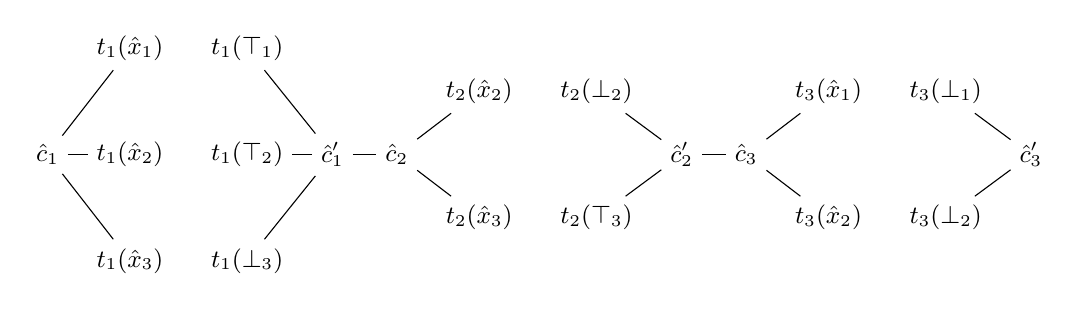
\begin{tikzpicture}[node distance=.3cm]
\small
\node(c1){$\hat{c}_1$};

\node[right =.25cm of c1] (t1x2) {$t_1(\hat{x}_2)$};
\node[above =.8cm of t1x2] (t1x1) {$t_1(\hat{x}_1)$};
\node[below =.8cm of t1x2] (f1x3) {$t_1(\hat{x}_3)$};
\draw [-] (c1) to (t1x2);
\draw [-] (c1) to (t1x1);
\draw [-] (c1) to (f1x3);

\node[right = 3.1cm of c1](c1p){$\hat{c}_1'$};

\node[left =.25cm of c1p] (t12) {$t_1(\top_2)$};
\node[above=.8cm of t12] (t11) {$t_1(\top_1)$};
\node[below=.8cm of t12] (f13) {$t_1(\bot_3)$};
\draw [-] (c1p) to (t11);
\draw [-] (c1p) to (t12);
\draw [-] (c1p) to (f13);

\node[right = .3cm of c1p](c2){$\hat{c}_2$};
\draw [-] (c1p) to (c2);

\node[right=.25cm of c2, yshift=.8cm]  (f2x2) {$t_2(\hat{x}_2)$};
\node[right=.25cm of c2, yshift=-.8cm] (t2x3) {$t_2(\hat{x}_3)$};
\draw [-] (c2) to (f2x2);
\draw [-] (c2) to (t2x3);

\node[right = 3.1cm of c2](c2p){$\hat{c}_2'$};
\node[left =.25cm of c2p, yshift=.8cm]  (f22) {$t_2(\bot_2)$};
\node[left =.25cm of c2p, yshift=-.8cm] (t23) {$t_2(\top_3)$};
\draw [-] (c2p) to (t23);
\draw [-] (c2p) to (f22);

\node[right = .3cm of c2p](c3){$\hat{c}_3$};
\draw [-] (c2p) to (c3);
\node[right =.25cm of c3, yshift=.8cm] (f3x1) {$t_3(\hat{x}_1)$};
\node[right =.25cm of c3, yshift=-.8cm] (f3x2) {$t_3(\hat{x}_2)$};
\draw [-] (c3) to (f3x1);
\draw [-] (c3) to (f3x2);

\node[right = 3.1cm of c3](c3p){$\hat{c}_3'$};
\node[left =.25cm of c3p, yshift=.8cm] (f31) {$t_3(\bot_1)$};
\node[left =.25cm of c3p, yshift=-.8cm] (f32) {$t_3(\bot_2)$};
\draw [-] (c3p) to (f31);
\draw [-] (c3p) to (f32);

\end{tikzpicture}


\caption{The congruence translation $E_{\mathcal{C}} = \Connect \cup \bigcup_{1 \leq i \leq n}\Clause_i$ of $\mathcal{C}$.}
\label{fig:npexamplebig}
\end{figure}

\end{example}

\begin{definition}[Assignment congruence translation]
\label{def:AssignmentCongruenceTranslation}
  The \emph{assignment congruence translation} $E_{\mathcal{I}}$ of an assignment $\mathcal{I}$ on propositional variables $x_1,\ldots,x_m$ is the set of equations
\begin{eqnarray*}
  E_{\mathcal{I}} & = & \phantom{\cup}\ \{ \hat{x}_j = \top_j \ \mid\  1 \leq j \leq m \text{ and } \mathcal{I} \models x_j \} \\
               &   & \cup\ \{ \hat{x}_j = \bot_j \ \mid\ 1 \leq j \leq m \text{ and } \mathcal{I} \models \neg x_j \}
\end{eqnarray*}
For convenience, we also define the set
\begin{equation*}
  \Assignment = \{ \hat{x}_j = \top_j, \hat{x}_j = \bot_j \ \mid\ 1 \leq j \leq m\}.
\end{equation*}
\end{definition}
\noindent
An assignment congruence translation is always a subset of
$\Assignment$.  By extension, a subset of $\Assignment$ is
said to be an assignment if it is the congruence translation of an assignment,
that is, if it does not contain both $\hat{x}_j = \top_j$ and $\hat{x}_j =
\bot_j$ for some $j$.

\begin{example}\label{ex:np2} (Example~\ref{ex:np1} continued)  
Consider the model $\mathcal{I} = \{x_1, \neg x_2, x_3\}$ of\/ $\mathcal{C}$.
Figure~\ref{fig:npassignment} gives a graphical representation of
$E_{\mathcal{I}}$, whereas $\Assignment$ is represented in
Figure~\ref{fig:npassignmentstar}.  Notice that
$E_{\mathcal{C}} \cup E_{\mathcal{I}} \models c_1 = c'_3$,
and $c_1$ and $c'_3$ are connected in the congruence graph
of $E_{\mathcal{C}} \cup E_{\mathcal{I}}$ (Figure~\ref{fig:npmodel}), the path containing both full edges corresponding to equalities in $E_{\mathcal{C}} \cup E_{\mathcal{I}}$, and dotted edged corresponding to equalities due to the compatibility property of the congruence relation.

\begin{figure}[ht]

\centering
\begin{tikzpicture}[node distance=1.5cm]

\node [below =.5cm of f2x2] (x1) {$\hat{x}_1$};
\node [below =.5cm of x1] (x2) {$\hat{x}_2$};
\node [below =.5cm of x2] (x3) {$\hat{x}_3$};

\node [right = of x1] (t1) {$\top_1$};

\draw [-] (x1) to (t1);

\node [left = of x2] (f2) {$\bot_2$};

\draw [-] (x2) to (f2);

\node [right = of x3] (t3) {$\top_3$};

\draw [-] (x3) to (t3);

\end{tikzpicture}


\caption{Congruence translation of $\mathcal{I}$}
\label{fig:npassignment}
\end{figure}

\begin{figure}[ht]

\centering
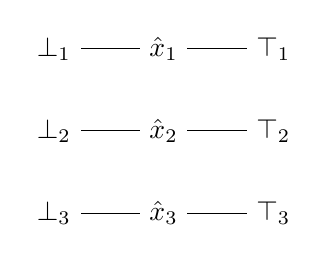
\begin{tikzpicture}[node distance=.75cm]

\node (x1) {$\hat{x}_1$};
\node [below =.5cm of x1] (x2) {$\hat{x}_2$};
\node [below =.5cm of x2] (x3) {$\hat{x}_3$};

\node [right = of x1] (t1) {$\top_1$};
\node [left = of x1] (f1) {$\bot_1$};

\draw [-] (x1) to (t1);
\draw [-] (x1) to (f1);

\node [right = of x2] (t2) {$\top_2$};
\node [left = of x2] (f2) {$\bot_2$};

\draw [-] (x2) to (t2);
\draw [-] (x2) to (f2);

\node [right = of x3] (t3) {$\top_3$};
\node [left = of x3] (f3) {$\bot_3$};

\draw [-] (x3) to (t3);
\draw [-] (x3) to (f3);

\end{tikzpicture}



\caption{$\Assignment$}
\label{fig:npassignmentstar}
\end{figure}

\begin{figure}[ht]

\centering
\begin{tikzpicture}[node distance=.3cm]
\small
\node(c1){$\hat{c}_1$};

\node[right =.25cm of c1] (t1x2) {$t_1(\hat{x}_2)$};
\node[above =.8cm of t1x2] (t1x1) {$t_1(\hat{x}_1)$};
\node[below =.8cm of t1x2] (t1x3) {$t_1(\hat{x}_3)$};
\draw [-] (c1) to (t1x2);
\draw [-] (c1) to (t1x1);
\draw [-] (c1) to (t1x3);

\node[right = 3.1cm of c1](c1p){$\hat{c}_1'$};

\node[left =.25cm of c1p] (t12) {$t_1(\top_2)$};
\node[above=.8cm of t12] (t11) {$t_1(\top_1)$};
\node[below=.8cm of t12] (t13) {$t_1(\bot_3)$};
\draw [-] (c1p) to (t11);
\draw [-] (c1p) to (t12);
\draw [-] (c1p) to (t13);

\node[right = .3cm of c1p](c2){$\hat{c}_2$};
\draw [-] (c1p) to (c2);

\node[right=.25cm of c2, yshift=.8cm]  (t2x2) {$t_2(\hat{x}_2)$};
\node[right=.25cm of c2, yshift=-.8cm] (t2x3) {$t_2(\hat{x}_3)$};
\draw [-] (c2) to (t2x2);
\draw [-] (c2) to (t2x3);

\node[right = 3.1cm of c2](c2p){$\hat{c}_2'$};
\node[left =.25cm of c2p, yshift=.8cm]  (t22) {$t_2(\bot_2)$};
\node[left =.25cm of c2p, yshift=-.8cm] (t23) {$t_2(\top_3)$};
\draw [-] (c2p) to (t23);
\draw [-] (c2p) to (t22);

\node[right = .3cm of c2p](c3){$\hat{c}_3$};
\draw [-] (c2p) to (c3);
\node[right =.25cm of c3, yshift=.8cm] (t3x1) {$t_3(\hat{x}_1)$};
\node[right =.25cm of c3, yshift=-.8cm] (t3x2) {$t_3(\hat{x}_2)$};
\draw [-] (c3) to (t3x1);
\draw [-] (c3) to (t3x2);

\node[right = 3.1cm of c3](c3p){$\hat{c}_3'$};
\node[left =.25cm of c3p, yshift=.8cm] (t31) {$t_3(\bot_1)$};
\node[left =.25cm of c3p, yshift=-.8cm] (t32) {$t_3(\bot_2)$};
\draw [-] (c3p) to (t31);
\draw [-] (c3p) to (t32);

\node [below =1.3cm of c2, xshift=1.5cm] (x1) {$\hat{x}_1$};
\node [below =.5cm of x1] (x2) {$\hat{x}_2$};
\node [below =.5cm of x2] (x3) {$\hat{x}_3$};

\node [right = of x1] (t1) {$\top_1$};

\draw [-] (x1) to (t1);

\node [left = of x2] (t2) {$\bot_2$};

\draw [-] (x2) to (t2);

\node [right = of x3] (t3) {$\top_3$};

\draw [-] (x3) to (t3);

\draw [dotted] (t1x1) to (t11);
\draw [dotted] (t1x3) to (t13);
\draw [dotted] (t2x2) to (t22);
\draw [dotted] (t2x3) to (t23);
\draw [dotted] (t3x2) to (t32);

\end{tikzpicture}


\caption{The congruence graph for $E_{\mathcal{C}} \cup E_{\mathcal{I}}$}
\label{fig:npmodel}
\end{figure}
\end{example}

\begin{lemma}
\label{lemma:eqv}
Consider a (partial or total) assignment $\mathcal{I}$ for non-tautological
clauses $\mathcal{C}= \{C_1, \dots C_n\}$.  Then $\mathcal{I} \models
\mathcal{C}$ if and only if $E_{\mathcal{I}} \cup E_\mathcal{C} \models c_1 =
c'_n$.
\end{lemma}
\begin{proof}

Let the propositional variables in $\mathcal{C}$ be $x_1,\ldots, x_m$.

($\Leftarrow$)  Consider the congruence graph induced by
$E_{\mathcal{I}} \cup E_\mathcal{C}$.  Besides edges directly associated to
equalities in the set, the only edges are congruence edges between terms
$t_i(\hat{x}_j)$ and either $t_i(\top_j)$ or $t_i(\bot_j)$.  So any path from
$c_1$ to $c'_n$ would go through such a congruence edge for each $i$.
And such an edge exists for $i$ if and only if the clause $i$ is satisfied by
$\mathcal{I}$.

($\Rightarrow$)  If $\mathcal{I} \models \mathcal{C}$, then
$\mathcal{I} \models C_i$ for each clause $C_i \in \mathcal{C}$.  Assume
$\mathcal{I}$ makes true a variable $x_j$, literal of $C_i$ (the case of
the negation of a variable is handled similarly).  Then $E_{\mathcal{I}} \models
t_i(\hat{x}_j) = t_i(\top_j)$, and $E_{\mathcal{I}} \cup \Clause_i
\models c_i = c_i'$.  This is true for each $i$, and
thanks to the equations in \Connect, one can deduce using transitivity that
$E_{\mathcal{I}} \cup E_\mathcal{C} \models c_1 = c_n'$.
\qed
\end{proof}

\begin{lemma}
Consider a (partial or total) assignment $\mathcal{I}$ for 
non-tautological clauses $\mathcal{C}= \{C_1, \dots C_n\}$ on variables  $x_1,\ldots, x_m$. $|E_{\mathcal{I}} \cup E_\mathcal{C}|$ and
$|\mathcal{T}(E_{\mathcal{I}} \cup E_\mathcal{C})|$ are polynomial in $n$ and
$m$.
\end{lemma}

\begin{proof}
$E_{\mathcal{I}}$ contains at most $m$ equations, since for no $j$ both $\mathcal{I} \models x_j$ and $\mathcal{I} \models \neg x_j$.
The set $\Connect$ contains exactly $n-1$ equations.
For every $i$, the set $\Clause_i$ contains at most $2m$ equations, resulting in $2mn$ equations for all clauses.
In total, we thus have $|E_{\mathcal{I}} \cup E_\mathcal{C}| \leq n-1 + m + 2mn$.

$E_{\mathcal{I}} \cup E_\mathcal{C}$ contains at most $2n + 3m + 3mn$ terms: $2n$ for $c_i,c_i'$, $3m$ for $\hat{x}_j,\top_j,\bot_j$ and $3mn$ for all possible combinations of $t_i(\hat{x}_j),t_i(\top_j),t_i(\bot_j)$.
\qed
\end{proof}

\noindent 
%Notice also that, for any model $\mathcal{I}$ of a set of $n$ clauses
%$\mathcal{C}$, every explanation that $E_{\mathcal{I}} \cup E_\mathcal{C}
%\models c_1 = c_n'$ contains at least two equalities in
%each set $\Clause_i$, since each clause has to be satisfied.  But also, there is
%an explanation that contains exactly two equalities in each set $\Clause_i$.
Considering again Example~\ref{ex:np2}, and particularly
Figure~\ref{fig:npmodel}, any transitivity chain from $c_1$ to
$c'_3$ will pass through $c'_1$, $c_2$, $c_2'$ and
$c_3$.  Any acyclic path from $c_1$ to $c'_3$ will contain 11
edges: 3 congruence edges, $3*2$ edges in $\Clause_i$ for $i=1,2,3$
and 2 edges from $\Connect$.

Since every interpretation $\mathcal{I}$ is such that $E_{\mathcal{I}} \subset
\Assignment$, one can try to relate the propositional satisfiability
problem for a set of clauses $\mathcal{C}= \{C_1, \dots C_n\}$ to finding an
explanation of $c_1 = c_n'$ in $\Assignment \cup
E_{\mathcal{C}}$.  However, it is necessary that this explanation does not set
$\hat{x}_j$ equal both to $\top_j$ and $\bot_j$, i.e.\ at most one of the two
equations $\hat{x}_j = \top_j$ and $\hat{x}_j = \bot_j$ should be in the
explanation.  By restricting assignments to total ones, i.e.\ by enforcing that
at least one of the two equations $\hat{x}_j = \top_j$ and $\hat{x}_j = \bot_j$
belongs to the explanation, it is also possible, with a single cardinality
condition on the explanation size, to require that at most one of them 
belong to the explanation.


\begin{lemma}
\label{lemma:satreduction}
A set of non-tautological clauses $\mathcal{C}= \{C_1, \dots C_n\}$ using
variables $x_1,\dots, x_m$ is satisfiable if and only if there is a set $E'$ such that $E'
\subseteq \Assignment \cup E_{\mathcal{C}'}$, $E'\models
c_1~=~c'_{n+m}$ and $|E'| \leq 3n+4m-1$, where $\mathcal{C}'$ is
$\mathcal{C}$ augmented with the tautological clauses $C_{n+i}~=~x_i \vee \neg
x_i$ for $i=1,\dots m$.
\end{lemma}
\begin{proof}
($\Rightarrow$)  Consider a total model $\mathcal{I}$ for $\mathcal{C}$.
We show that there is a set $E \subset E_{\mathcal{C}'}$, such that together with the congruence translation $E_{\mathcal{I}}$ of $\mathcal{I}$ it follows $E'~=~E \cup E_{\mathcal{I}} \models c_1~=~c'_{n+m}$ and $|E'| \leq 3n+4m-1$.

The set $E_{\mathcal{I}}$ contains $m$ equations, since it is the congruence translation of a total assignment.

For each clause $C_i$ ($i= 1\dots n + m$), there is a literal in $C_i$ that is satisfied by the model $\mathcal{I}$.
Let $x_j$ be the variable of that literal.

Suppose $\mathcal{I} \models x_j$, then the set $E$ contains equations $c_i~=~t_i(\hat{x}_j), t_i(\top_j)~=~c'_i$ of $Clause_i$.
These equations are in $Clause_i$, because $x_j$ is the satisfying literal of $C_i$, thus surely $x_j \in C_i$.
From compatibility and the fact that $\hat{x}_j~=~\top_j~\in~E_{\mathcal{I}}$ it follows that $E \cup E_{\mathcal{I}} \models t_i(\hat{x}_j)~=~t_i(\top_j)$.
Finally, from transitivity and the three equations $c_i~=~t_i(\hat{x}_j)$, $t_i(\hat{x}_j)~=~t_i(\top_j)$, $t_i(\top_j)~=~c'_i$ it follows that $E \cup E_{\mathcal{I}} \models c_i~=~c'_i$.

The case $\mathcal{I} \not\models x_j$ is symmetric, such that via equations $c_i~=~t_i(\hat{x}_j)$,  $t_i(\hat{x}_j)~=~t_i(\bot_j)$, $t_i(\bot_j)~=~c'_i$, it follows $E \cup E_{\mathcal{I}} \models c_i~=~c'_i$.

In addition to $2$ equations for each of the $(n~+~m)$ clauses, the set $E$ contains all $n + m - 1$ equations of $\Connect$, that is $c'_i~=~c_{i+1}$ for $i~=~1\dots n + m - 1$.
From transitivity it follows that $E \cup E_{\mathcal{I}} \models c_1~=~c'_{n+m}$.

In total, $E$ contains $2(n~+~m)$ of the sets $Clause_i$, $n+m-1$ equations from $\Connect$ and $m$ equations from $E_{\mathcal{I}}$, i.e. $|E|~=~3n + 4m - 1$.

($\Leftarrow$) 
Suppose there is a set of equations $E' \subseteq \Assignment \cup E_{\mathcal{C}'}$ such that $E'\models c_1~=~c'_{n+m}$ and $|E'| \leq 3n+4m-1$.
$E'$ has to contain $2(n~+~m)$ equations from $\Clause_i$ 
($i= 1\dots n + m$), that is one pair of equations $c_i~=~t_i(.)$ and $t_i(.)~=~c'_i$ for every clause, and $n + m - 1$ equations from $\Connect$, since by construction there is no other possibility to deduce $c_i~=~c'_i$.
Furthermore, thanks to the tautological
clauses, $E'$ also has to contain at least $\hat{x}_j~=~\top_j$ or
$\hat{x}_j~=~\bot_j$ for each $j\in\{1\dots m\}$.  
Therefore, the cardinality
condition $|E'| \leq 3n+4m-1$ and the fact that $E'$ contains $3(n~+~m) - 1$ equations from $Clause_i$ and $\Connect$, requires that the $E'$ contains at most one $\hat{x}_j =
\top_j$ or $\hat{x}_j~=~\bot_j$ for each $j\in\{1\dots m\}$.
Therefore, we have that $E_{\mathcal{I}}~=~E' \cap \Assignment$ is the congruence translation of an assignment and Lemma~\ref{lemma:eqv} guarantees the existence of a model
for $\mathcal{C'}$, or equivalently for the original set of clauses
$\mathcal{C}$.
\qed
\end{proof}

\begin{example}

In Lemma \ref{lemma:satreduction}, we add tautological clauses to the input formula.
We demonstrate the necessity of these extra clauses on the unsatisfiable formula $\varphi = (x_1 \vee x_2) \wedge (\neg x_1 \vee x_2) \wedge (x_1 \vee \neg x_2) \wedge (\neg x_1 \vee \neg x_2)$.
%
% Old version:
% ============
% Figure \ref{fig:spurious} shows the congruence translation of $\varphi$ together with a subset of $\Assignment$ that yields a short explanation for $c_1 = c_4'$.
% This short explanation corresponds to mapping $x_1$ to $\bot$ and $\top$ at the same time, which clearly is not the translation of an assignment.
% By short, we mean an explanation that, on top of necessary equations from the clause and connect parts, picks $m$ equations from the $\Assignment$ part.
%
% Figure \ref{fig:withtautol} shows the congruence translation of $\varphi$ conjoined with the tautological clauses $(x_1 \vee \neg x_1)$ and $(x_2 \vee \neg x_2)$, together with the same subset of $\Assignment$ that was a short explanation before.
% It is not an explanation of $c_1 = c_6'$, since the transitivity chain stops at $t_6(\hat{x}_2)$.
% In this congruence graph, there is no spurious short explanation of $c_1 = c_6'$ that does not correspond to an assignment.
% This is the desired result, because $\varphi$ is unsatisfiable.
%
Figure \ref{fig:spurious} shows the congruence translation of $\varphi$ together with a subset of $\Assignment$ that yields an explanation for $c_1 = c_4'$ that picks, besides the necessary equations from the clause and connect parts, $m$ equations from the $\Assignment$ part.
However, this explanation maps $x_1$ to $\bot$ and $\top$ at the same time, and hence cannot correspond to a (consistent) assignment. With the addition of tautological clauses, spurious explanations of this kind are blocked. This is shown in Figure \ref{fig:withtautol}, depicting the congruence translation of $\varphi$ conjoined with the tautological clauses $(x_1 \vee \neg x_1)$ and $(x_2 \vee \neg x_2)$, together with the same subset of $\Assignment$ used in Figure \ref{fig:spurious}. As desired, this subset is not an explanation of $c_1 = c_6'$, since the transitivity chain stops at $t_6(\hat{x}_2)$.
In fact, in this congruence graph, there is no spurious explanation of $c_1 = c_6'$. More generally, as desired, there cannot be any explanation of $c_1 = c_6'$, because $\varphi$ is unsatisfiable.





\begin{figure}[htb]

\centering
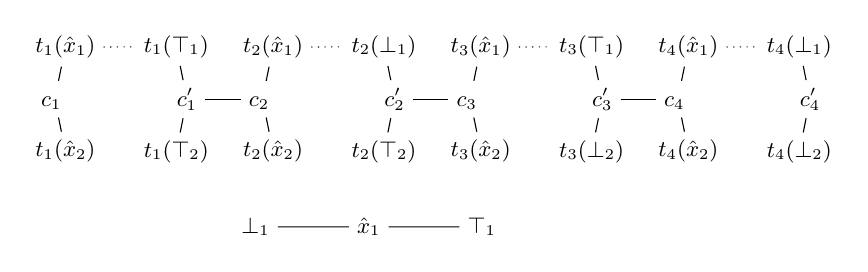
\begin{tikzpicture}[scale=0.9, every node/.style={transform shape}]
\small
\node(c1){$c_1\phantom{'}$};

\node[below =.2cm of c1,xshift=.15cm] (t1x2) {$t_1(\hat{x}_2)$};
\node[above =.2cm of c1,xshift=.15cm] (t1x1) {$t_1(\hat{x}_1)$};
\draw [-] (c1) to (t1x2);
\draw [-] (c1) to (t1x1);

\node[right = 1.3cm of c1](c1p){$c_1'$};

\node[below =.2cm of c1p,xshift=-.15cm] (t12) {$t_1(\top_2)$};
\node[above =.2cm of c1p,xshift=-.15cm] (t11) {$t_1(\top_1)$};
\draw [-] (c1p) to (t11);
\draw [-] (c1p) to (t12);

\node[right = .5cm of c1p](c2){$c_2\phantom{'}$};
\draw [-] (c1p) to (c2);

\node[below =.2cm of c2,xshift=.15cm] (t2x2) {$t_2(\hat{x}_2)$};
\node[above =.2cm of c2,xshift=.15cm] (t2x1) {$t_2(\hat{x}_1)$};
\draw [-] (c2) to (t2x2);
\draw [-] (c2) to (t2x1);

\node[right = 1.3cm of c2](c2p){$c_2'$};

\node[below =.2cm of c2p,xshift=-.15cm] (t22) {$t_2(\top_2)$};
\node[above =.2cm of c2p,xshift=-.15cm] (t21) {$t_2(\bot_1)$};
\draw [-] (c2p) to (t21);
\draw [-] (c2p) to (t22);

\node[right = .5cm of c2p](c3){$c_3\phantom{'}$};
\draw [-] (c2p) to (c3);

\node[below =.2cm of c3,xshift=.15cm] (t3x2) {$t_3(\hat{x}_2)$};
\node[above =.2cm of c3,xshift=.15cm] (t3x1) {$t_3(\hat{x}_1)$};
\draw [-] (c3) to (t3x2);
\draw [-] (c3) to (t3x1);

\node[right = 1.3cm of c3](c3p){$c_3'$};

\node[below =.2cm of c3p,xshift=-.15cm] (t32) {$t_3(\bot_2)$};
\node[above =.2cm of c3p,xshift=-.15cm] (t31) {$t_3(\top_1)$};
\draw [-] (c3p) to (t31);
\draw [-] (c3p) to (t32);

\node[right = .5cm of c3p](c4){$c_4\phantom{'}$};
\draw [-] (c3p) to (c4);

\node[below =.2cm of c4,xshift=.15cm] (t4x2) {$t_4(\hat{x}_2)$};
\node[above =.2cm of c4,xshift=.15cm] (t4x1) {$t_4(\hat{x}_1)$};
\draw [-] (c4) to (t4x2);
\draw [-] (c4) to (t4x1);

\node[right = 1.3cm of c4](c4p){$c_4'$};

\node[below =.2cm of c4p,xshift=-.15cm] (t42) {$t_4(\bot_2)$};
\node[above =.2cm of c4p,xshift=-.15cm] (t41) {$t_4(\bot_1)$};
\draw [-] (c4p) to (t41);
\draw [-] (c4p) to (t42);

\node [below =1.3cm of c2, xshift=1.5cm] (x1) {$\hat{x}_1$};
\node [right = of x1] (t1) {$\top_1$};
\draw [-] (x1) to (t1);

\node [left = of x1] (f1) {$\bot_1$};
\draw [-] (x1) to (f1);

\draw [dotted] (t1x1) to (t11);
\draw [dotted] (t2x1) to (t21);
\draw [dotted] (t3x1) to (t31);
\draw [dotted] (t4x1) to (t41);

\end{tikzpicture}


\caption{The congruence translation of $\varphi$ and a spurious short explanation.}
\label{fig:spurious}
\end{figure}

\begin{figure}[htb]

\centering
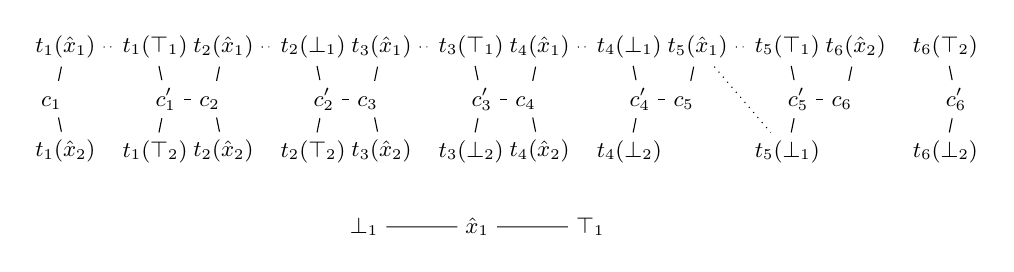
\begin{tikzpicture}[scale=0.9, every node/.style={transform shape}]
\small
\node(c1){$c_1\phantom{'}$};

\node[below =.2cm of c1,xshift=.15cm] (t1x2) {$t_1(\hat{x}_2)$};
\node[above =.2cm of c1,xshift=.15cm] (t1x1) {$t_1(\hat{x}_1)$};
\draw [-] (c1) to (t1x2);
\draw [-] (c1) to (t1x1);

\node[right = 1cm of c1](c1p){$c_1'$};

\node[below =.2cm of c1p,xshift=-.15cm] (t12) {$t_1(\top_2)$};
\node[above =.2cm of c1p,xshift=-.15cm] (t11) {$t_1(\top_1)$};
\draw [-] (c1p) to (t11);
\draw [-] (c1p) to (t12);

\node[right = .1cm of c1p](c2){$c_2\phantom{'}$};
\draw [-] (c1p) to (c2);

\node[below =.2cm of c2,xshift=.15cm] (t2x2) {$t_2(\hat{x}_2)$};
\node[above =.2cm of c2,xshift=.15cm] (t2x1) {$t_2(\hat{x}_1)$};
\draw [-] (c2) to (t2x2);
\draw [-] (c2) to (t2x1);

\node[right = 1cm of c2](c2p){$c_2'$};

\node[below =.2cm of c2p,xshift=-.15cm] (t22) {$t_2(\top_2)$};
\node[above =.2cm of c2p,xshift=-.15cm] (t21) {$t_2(\bot_1)$};
\draw [-] (c2p) to (t21);
\draw [-] (c2p) to (t22);

\node[right = .1cm of c2p](c3){$c_3\phantom{'}$};
\draw [-] (c2p) to (c3);

\node[below =.2cm of c3,xshift=.15cm] (t3x2) {$t_3(\hat{x}_2)$};
\node[above =.2cm of c3,xshift=.15cm] (t3x1) {$t_3(\hat{x}_1)$};
\draw [-] (c3) to (t3x2);
\draw [-] (c3) to (t3x1);

\node[right = 1cm of c3](c3p){$c_3'$};

\node[below =.2cm of c3p,xshift=-.15cm] (t32) {$t_3(\bot_2)$};
\node[above =.2cm of c3p,xshift=-.15cm] (t31) {$t_3(\top_1)$};
\draw [-] (c3p) to (t31);
\draw [-] (c3p) to (t32);

\node[right = .1cm of c3p](c4){$c_4\phantom{'}$};
\draw [-] (c3p) to (c4);

\node[below =.2cm of c4,xshift=.15cm] (t4x2) {$t_4(\hat{x}_2)$};
\node[above =.2cm of c4,xshift=.15cm] (t4x1) {$t_4(\hat{x}_1)$};
\draw [-] (c4) to (t4x2);
\draw [-] (c4) to (t4x1);

\node[right = 1cm of c4](c4p){$c_4'$};

\node[below =.2cm of c4p,xshift=-.15cm] (t42) {$t_4(\bot_2)$};
\node[above =.2cm of c4p,xshift=-.15cm] (t41) {$t_4(\bot_1)$};
\draw [-] (c4p) to (t41);
\draw [-] (c4p) to (t42);

\node[right = .1cm of c4p](c5){$c_5\phantom{'}$};
\draw [-] (c4p) to (c5);

\node[above =.2cm of c5,xshift=.15cm] (t5x1) {$t_5(\hat{x}_1)$};
\draw [-] (c5) to (t5x1);

\node[right = 1cm of c5](c5p){$c_5'$};

\node[below =.2cm of c5p,xshift=-.15cm] (t52) {$t_5(\bot_1)$};
\node[above =.2cm of c5p,xshift=-.15cm] (t51) {$t_5(\top_1)$};
\draw [-] (c5p) to (t51);
\draw [-] (c5p) to (t52);

\node[right = .1cm of c5p](c6){$c_6\phantom{'}$};
\draw [-] (c5p) to (c6);

\node[above =.2cm of c6,xshift=.15cm] (t6x2) {$t_6(\hat{x}_2)$};
\draw [-] (c6) to (t6x2);

\node[right = 1cm of c6](c6p){$c_6'$};

\node[below =.2cm of c6p,xshift=-.15cm] (t62) {$t_6(\bot_2)$};
\node[above =.2cm of c6p,xshift=-.15cm] (t61) {$t_6(\top_2)$};
\draw [-] (c6p) to (t61);
\draw [-] (c6p) to (t62);

\node [below =1.3cm of c3, xshift=1.5cm] (x1) {$\hat{x}_1$};
\node [right = of x1] (t1) {$\top_1$};
\draw [-] (x1) to (t1);

\node [left = of x1] (f1) {$\bot_1$};
\draw [-] (x1) to (f1);

\draw [dotted] (t1x1) to (t11);
\draw [dotted] (t2x1) to (t21);
\draw [dotted] (t3x1) to (t31);
\draw [dotted] (t4x1) to (t41);
\draw [dotted] (t5x1) to (t51);
\draw [dotted] (t5x1) to (t52);

\end{tikzpicture}


\caption{The congruence translation of $\varphi$ with tautological clauses.}
\label{fig:withtautol}
\end{figure}

\end{example}

\begin{corollary}[NP-hardness]
\label{lemma:nphardness}
The small explanation problem is NP-hard.
\end{corollary}
\begin{proof}
Propositional satisfiability is NP-hard, and can be reduced in polynomial time to the small explanation problem.
\qed
\end{proof}

\begin{lemma}[NP]
\label{lemma:innp}
The small explanation problem is in NP.
\end{lemma}
\begin{proof}
Let $E$ be a set of equations and $s=t$ be a target equation.
A solution to the explanation problem for some $k \in \mathbb{N}$ is a subset $E' \subseteq E$, such that $|E'| \leq k$.
Let $n = |\mathcal{T}(E)| + |E|$ and $n' = |\mathcal{T}(E')| + |E'|$.
We have $n' \leq n$, since $E' \subseteq E$ and every term in $E'$ appears also in $E$.
Checking whether $E'$ is an explanation of $s=t$ can be done by computing its congruence closure, which is possible in polynomial time in $n'$ \cite{Nelson2} and thereby also in $n$.
\qed
\end{proof}


\begin{theorem}[Small explanation NP-completeness]
The small explanation problem is NP-complete.
\end{theorem}
\begin{proof}
By corollary~\ref{lemma:nphardness} and lemma~\ref{lemma:innp}.
\qed
\end{proof}

\begin{theorem}[Small conflict NP-completeness]
The small conflict set problem is NP-complete.
\end{theorem}
\begin{proof}
The small conflict set problem is at least as hard as the small explanation problem since the small explanation problem has been showed to be reducible to the small conflict set problem.  It is also in NP for exactly the same reason that the small explanation problem is.
\qed
\end{proof}


\section{Conclusion}

%\marginpar{Besson PxTP}
The conflict set generation feature of congruence algorithms is essential for
practical SMT solving.  Although one could argue that the important property of the generated conflicts is minimality (i.e.\ no useless literal is in the conflict), it is also interesting to consider producing the smallest conflict.  We have shown that the problem of deciding whether a conflict of a given size exists is NP-complete. Therefore, it is generally intractable to obtain the smallest conflict. 

In \cite{Fontaine1,Nieuwenhuis3,Nieuwenhuis9}, methods to obtain small
conflicts, but not necessarily the smallest, are discussed.  In practice, it
pays off to prioritize speed of the congruence closure algorithm and conflict
generation over succinctness of conflicts.  However, other applications
sensitive to proof size may benefit from other methods prioritizing small
conflict size, at a cost of less efficient solving. Thanks to the
NP-completeness, one option could be to iteratively encode the small conflict
problem into SAT, and use a SAT-solver to find successively smaller conflicts,
until the smallest is found. 
Perhaps an encoding of the problem can be found that differentiates between hard constraints representing relevant instantiations of the axioms of equality as well as the target equation,
and soft constraints representing the inclusion of input equations to an explanation.
In that case, Max-SAT solvers could be used to find small explanations, 
in order to leverage efforts that combine decision procedures and optimization techniques. %\cite{schiex1995valued,davies2013solving}.
%to avoid repeated calls to the SAT-solver and find the smallest conflict in one run.
%\marginpar{note that we would have to encode and call a SAT-solver many times, with progressively smaller values of $k$, until we find a value of $k$ for which the encoded problem is unsatisfiable. this would guarantee a \emph{minimum} conflict, but would probably be less efficient than the iterative addition/removal of literals from the explanation, which only guarantees a \emph{minimal} conflict.} 

\vspace*{5pt}\noindent {\bf Acknowledgment.} We would like to thank Robert
Nieuwenhuis and Ashish Tiwari for discussions and some preliminary ideas that
led us to this proof.  We are grateful to the anonymous reviewers of this paper
and of~\cite{Fellner1} for their comments.

% Sorry but the spbasic style is not looking great
\bibliographystyle{plain}
%\bibliographystyle{spbasic}
\bibliography{biblio}

\end{document}
